\chapter{Circular Waveguide (1)}\label{lec:lec44}
In the previous chapter, we discussed the second-order partial differential equation (PDE) of the form given in equation~\eqref{eqn:secondorderode} called the \emph{Bessel equation}\label{bessel equation}. It is given as
\begin{equation*}
x^2\derivative[2]{y}{x} + x\derivative{y}{x} + (x^2-n^2)y = 0
\end{equation*}
There is one kind of solution called the \emph{Bessel function\index{bessel function} of the first kind} which is an infinite series from equation~\eqref{eqn:besselsolnseries2} given as
\begin{equation*}
J_n(x) = \sum^\infty_{k=0} \frac{(-1)^k (\frac{x}{2})}{k!\Gamma(n+k+1)}
\end{equation*}
Where n is the order of the solution and $\Gamma(n+k+1) = (n+k)\Gamma(n+k)$. As we know for any second-order PDE there are always two different independent solutions and so we have another solution called the \emph{Bessel function of second kind} or Neumann function\index{neumann function} which from equation~\eqref{eqn:neumannfunctions} is given as 
\[
Y_n(x) = \frac{\cos(n\pi)J_n(x)-J_{-n}(x)}{\sin(n\pi)}
\]
In general, the solution of the Bessel equation is
\[
y(x) = A J_n(x) + B Y_n(x)
\]
However, $Y_n(0)=\pm\infty$ means at the centre of cylindrical symmetry, the electromagnetic fields or power density is infinite which makes no physical sense. So due to practical reasons, the solution of the Bessel function is 
\[
y(x) = A J_n(x)
\]
In addition to the Bessel functions of the first and second kind, there is another type known as the \emph{Bessel function of the third kind}, commonly referred to as the Henkel functions. These Henkel functions hold significance in the field of electromagnetics, particularly when dealing with dielectric waveguides like optical fibres. In the modelling of such structures, the Bessel function of the first kind is employed to describe the behaviour inside the waveguide, while the Bessel functions of the third kind (Henkel functions) are utilized to represent the behaviour outside the waveguide. This distinction allows for a comprehensive characterization of the wave propagation in dielectric waveguides.
 
For all electromagnetic problems, the order $n$ is always an integer. So we will have the following Bessel functions $ J_0(x), J_1(x), J_2(x), \ldots$ where only $J_0(x)$ has some value at $x=0$ while the rest have the value zero, mathematically, we say 
\[
J_n(0)=0\quad\text{for }n \neq 0
\]
When we plot these functions, we notice that their behaviour resembles that of the sine and cosine functions. This similarity arises from the fact that both types of functions are periodic. However, as the value of x increases, the peak value of the functions begins to diminish. For example, if we plot the Bessel function $J_0(x)$, as depicted in Figure~\ref{fig:fig1}, it reaches its maximum at x = 0 and experiences attenuation as x increases.
\begin{figure}[h]
\centering
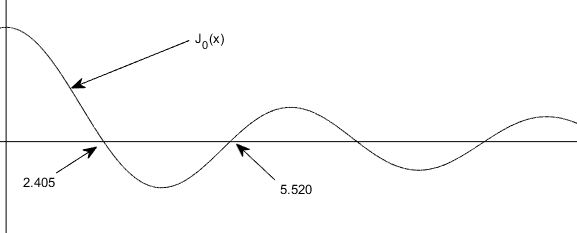
\includegraphics[width=1\linewidth]{\pathtoparttwo/graphics/fig_1.1}
\caption{Plot of Bessel function $J_0(x)$}
\label{fig:fig1}
\end{figure}

As we go to higher-order functions the behaviour is similar to a sine function. Let us plot the Bessel function $J_1(x)$ as shown in Figure~\ref{fig:fig2}.
\begin{figure}[h]
\centering
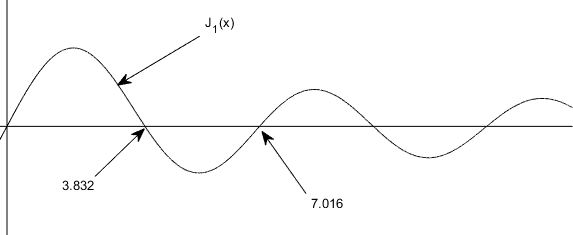
\includegraphics[width=1\linewidth]{\pathtoparttwo/graphics/fig_2.1}
\caption{Plot of Bessel function $J_1(x)$}
\label{fig:fig2}
\end{figure}

In the search for a solution to the waveguide, we encounter two constraints that must be taken into account:
\begin{enumerate}[(i)]
\item The first constraint pertains to the order $n$ of the solution. This order determines how the wave oscillates within the waveguide.
\item The second constraint, denoted by $p$, involves the selection of a specific zero point (root) of the electric field. It is necessary for the electric field to reach a zero point (root) at the boundary of the waveguide.
\end{enumerate}
By considering these two constraints, we are able to characterize the behaviour of the wave in the waveguide. The order $n$ governs the oscillation pattern, while the choice of zero point (root) $p$ determines the specific behaviour at the boundary. 

Consequently, we can denote the solution as $J_n^p(x)$, representing a distinct and particular solution. For each conceivable solution $J_n^p(x_{np})$, there exists a singular value of $x_{np}$ at which $J_n^p(x_{np})$ equals zero, as illustrated in Table~\ref{tab:table1}.
\begin{table}
\centering
\caption{Values of zeros in the Bessel functions of the first kind}
\begin{tabular}{|c|c c c|}
\hline 
\backslashbox{p}{n} & n=0 & n=1 & n=2 \\ 
\hline 
1&  2.405&  3.832& 5.136 \\ 
2&  5.520&  7.016& 8.417 \\ 
\hline 
\end{tabular}
\label{tab:table1}
\end{table}

The occurrence of cut-off frequencies in the circular waveguide can be observed from Table~\ref{tab:table1}. In the circular waveguide, the parameters $n$ and $p$ serve a similar purpose as $m$ and $n$ in the rectangular waveguide. They define the modes and corresponding cut-off frequencies for each mode. As a reminder from the rectangular waveguide, the value of 
$m$ represents the number of peaks in the x direction, while $n$ represents the number of peaks in the y direction. However, in the case of the circular waveguide, the arguments $n$ and $p$ indicate the order and root of the solution being considered.

In order to determine the solution for the circular waveguide, it is necessary to examine the derivative of the Bessel function. This derivative becomes crucial when applying the boundary conditions in the waveguide solution.

\section{TM mode in a Circular Waveguide}
Let us examine a hollow metallic pipe characterized by a radius of a. The interior of the pipe is filled with a dielectric material with respective permeability $\mu$ and permittivity $\epsilon$, as illustrated in Figure~\ref{fig:fig3}.
\begin{figure}[h]
\centering
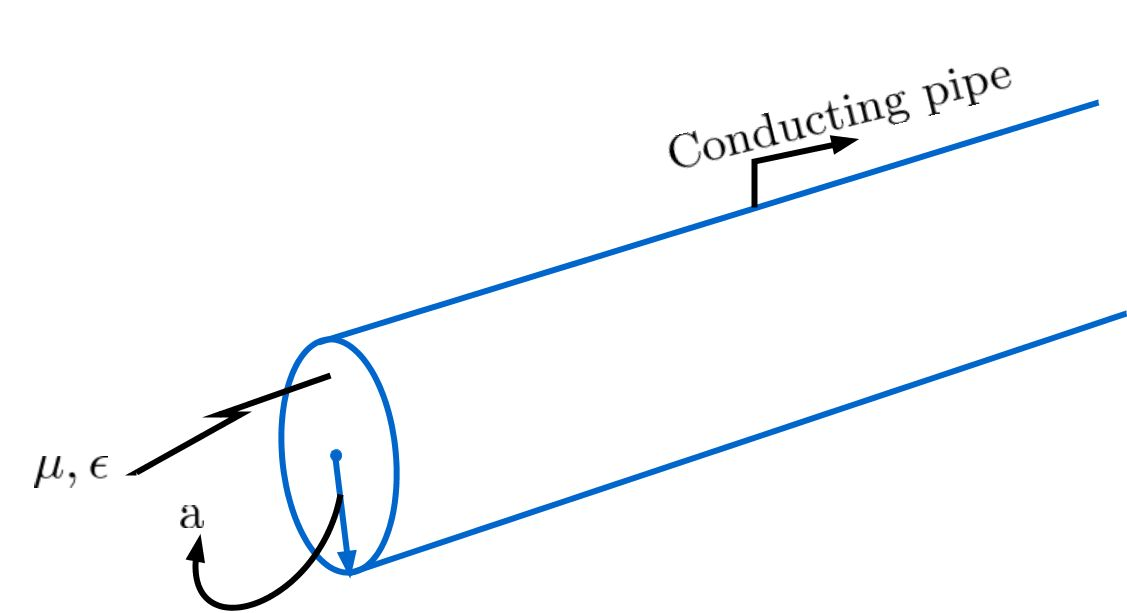
\includegraphics[width=0.7\linewidth]{\pathtoparttwo/graphics/fig_3.1}
\caption{Circular Waveguide of radius $a$ and dielectric material, $\mu, \epsilon$}
\label{fig:fig3}
\end{figure}

From the Helmholtz wave equation in equation~\eqref{eqn:helmholtzelectric} 
\begin{equation}
\nabla^2\vec{E} + \omega^2\mu\epsilon\vec{E}=0
\label{eqn:helmholtzelectriclec44}
\end{equation}\
The Laplacian operator $\nabla^2\vec{E}$ encompasses both transverse and longitudinal components. However, our focus lies on finding a solution of the form $\vec{E}=\vec{E}_{\bot}e^{-\gamma z}$, where the amplitude $\vec{E}_\bot$ remains confined to the transverse plane, and the wave propagates along the z-axis with a propagation constant denoted by $\gamma$. So we will write equation \ref{eqn:helmholtzelectriclec44} as
\begin{align*}
\nabla^2\vec{E}_\perp e^{-\gamma z} + \omega^2 \mu\epsilon E_\perp e^{-\gamma z} = 0\\\text{where }\nabla^2 = \nabla^2_\perp + \partialderivative[2]{}{z}&\\
\nabla^2_\perp\vec{E}_\perp e^{-\gamma z} + \partialderivative[2]{}{z}\left(\vec{E}_\perp e^{-\gamma z}\right) + \omega^2\mu\epsilon\vec{E}_\perp e^{-\gamma z} =&  0\\
\nabla^2_\perp\vec{E}_\perp e^{-\gamma z} + (\gamma^2)\left(\vec{E}_\perp e^{-\gamma z}\right) + \omega^2\mu\epsilon\vec{E}_\perp e^{-\gamma z} =& 0\\
\nabla^2_\perp\vec{E}_\perp e^{-\gamma z} + (\omega^2\mu\epsilon + \gamma^2)\left(\vec{E}_\perp e^{-\gamma z}\right) =& 0
\end{align*}
\begin{equation}
\nabla^2_\perp\vec{E}_\perp + (\omega^2\mu\epsilon + \gamma^2)\vec{E}_\perp = 0
\label{eqn:helmholtzelectriclec44_2}
\end{equation}
Where $h^2 = \omega^2\mu\epsilon + \gamma^2$. In order to solve Equation~\ref{eqn:helmholtzelectriclec44_2}, we will employ the cylindrical coordinate system. This choice is motivated by the circular nature of the waveguide's transverse plane, which exhibits radial symmetry. Unlike the rectangular waveguide, where the limits along the y-direction remained constant for any chosen location along the x-axis in the transverse plane, the circular waveguide's y-limits vary depending on the x-coordinate. Hence, utilizing the cylindrical coordinate system is preferable for solving the equation due to the cylindrical symmetry inherent in the waveguide's geometry.
 
The cylindrical coordinate system is defined by $\hat{r}$ and $\hat{\phi}$ in the transverse plane and $\hat{z}$ in the longitudinal direction.
\begin{figure}[h]
\centering
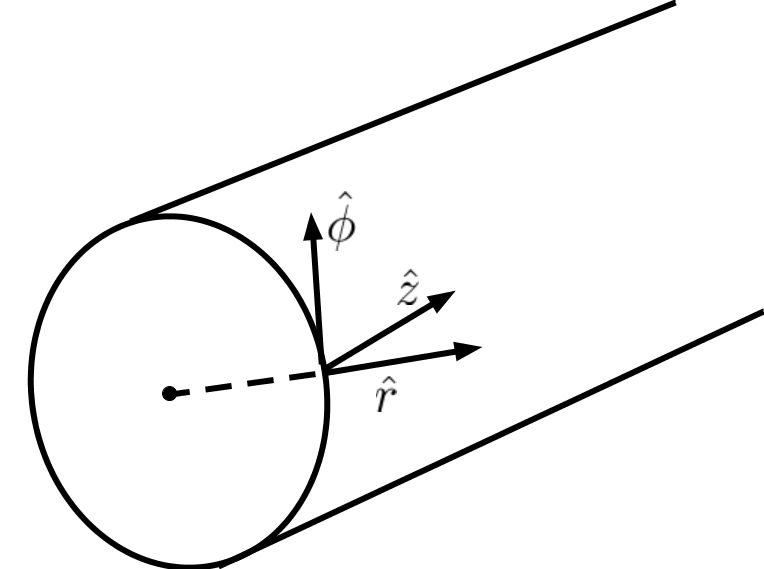
\includegraphics[width=0.7\linewidth]{\pathtoparttwo/graphics/fig_4.1}
\caption{Cylindrical coordinates for the circular waveguide}
\label{fig:fig4}
\end{figure}

We will now write equation \ref{eqn:helmholtzelectriclec44_2} for the cylindrical coordinate as 
\begin{align}
\frac{1}{r}\partialderivative{}{r}\left(r\partialderivative[2]{\vec{E}_\bot}{r}\right) + \frac{1}{r^2}\partialderivative[2]{\vec{E}_\bot}{\phi}+ h^2\vec{E}_\bot = 0 
\label{eqn:cylindricalequation}   
\end{align}
This is the equation which will give the solution of the modes. The field components in the circular waveguide are $E_r$, $E_\phi$ and $E_z$ as shown in Figure~\ref{fig:fig5}
\begin{figure}[h]
\centering
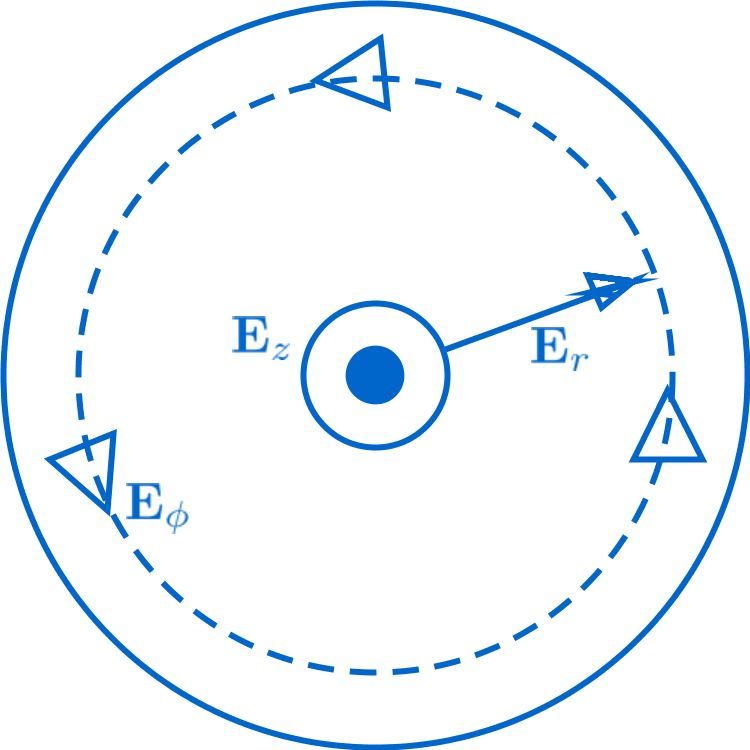
\includegraphics[width=0.5\linewidth]{\pathtoparttwo/graphics/fig_5.1}
\caption{Field components in the circular waveguide}
\label{fig:fig5}
\end{figure}

For the TM mode, we know that $H_z=0$ and $E_z$ exist and for the TE mode, $E_z=0$ and $H_z$ will exist. Therefore, for the TM mode, we should solve for $E_z$ with appropriate boundary conditions and for the TE mode, we should solve for $H_z$ with appropriate boundary conditions. 

So for the TM mode, we will solve for $E_z$ which should vary in $r$ and $\phi$ and propagates in the z direction, that is,
\begin{align*}
E_z(r,\phi, z)=E_z(r,\phi)e^{-\gamma z}\quad\text{where }e^{-\gamma z}
\end{align*}
It signifies the field is propagating in the z-direction. So from the from equation~\eqref{eqn:cylindricalequation} we have;
\begin{equation}
\frac{1}{r}\partialderivative{}{r}\left(r\partialderivative{E_z}{r}\right) + \frac{1}{r^2}\partialderivative[2]{E_z}{\phi} + h^2 E_z = 0 
\label{eqn:pdecircularwaveguide}
\end{equation}
Also, it is important to note that the variables $r$ and $\phi$ are orthogonal to each other, as depicted in Figure~\ref{fig:fig4}. This implies that any variation in the radial coordinate $r$ is independent of the variations in the azimuthal coordinate $\phi$. Hence, we can express $E_z$ as a function of $r$ and $\phi$ in the following manner:
\begin{align*}
E_z(r, \phi) = R(r)\Phi(\phi)\footnotemark
\end{align*}
\footnotetext{
Using separation of variables where $R(r)$ is a function of $r$ only and $\Phi(\phi)$ is a function of $\phi$ only.
}

So we will write equation \ref{eqn:pdecircularwaveguide} as 
\begin{align*}
&\frac{1}{r}\partialderivative{}{r}\left(r\partialderivative{R(r)\Phi(\phi)}{r}\right) + \frac{1}{r^2}\partialderivative[2]{R(r)\Phi(\phi)}{\phi} + h^2E_z(r,\phi) = 0\\
&\frac{\Phi(\phi)}{r}\derivative{}{r}\left(r\derivative{R(r)}{r}\right) + \frac{R}{r^2}\derivative[2]{\Phi(\phi)}{\phi} + h^2 E_z = 0\\
&\text{Divide through by }E_z(r,\phi)=R(r)\Phi(\phi)&\\
&\frac{1}{rR(r)}\derivative{}{r}\left(r\derivative{R(r)}{r}\right) + \frac{1}{r^2\Phi(\phi)}\derivative[2]{\Phi(\phi)}{\phi} + h^2 = 0\\
&\text{Multiply through by }r^2\\
&\frac{r}{R(r)}\derivative{}{r}\left(r\derivative{R(r)}{r}\right) + \frac{1}{\Phi(\phi)}\derivative[2]{\Phi(\phi)}{\phi} + r^2h^2 = 0
\end{align*}
\begin{dmath}
\underbrace{\frac{r}{R(r)}\derivative{}{r}\left(r\derivative{R(r)}{r}\right) + r^2 h}_{\text{function of }r\text{ only}} 
+ \underbrace{\frac{1}{\Phi(\phi)}\derivative[2]{\Phi(\phi)}{\phi}}_{\text{function of }\phi\text{ only}} = 0 
\label{eqn:pdecircularwaveguide2} 
\end{dmath}
Equation~\eqref{eqn:pdecircularwaveguide2} is true for any value of $r$ and $\phi$ and can only be true if each function is a constant. Let us denote that constant as $-n^2$ for the function of $\phi$ only i.e. 
\begin{align*}
\frac{1}{\Phi(\phi)}\derivative[2]{\Phi(\phi)}{\phi}=-n^2\quad\text{which implies that}
\end{align*}
\begin{equation}
\derivative[2]{\Phi(\phi)}{\phi} + n^2\Phi(\phi) = 0
\label{eqn:pdecircularwaveguide3}
\end{equation}
And so $\frac{r}{R(r)}\derivative{}{r}\left(r\derivative{R(r)}{r}\right) + r^2 h$ has to be $+n^2$ so that equation~\eqref{eqn:pdecircularwaveguide2} holds true, hence;
\begin{align*}
\underbrace{\frac{r}{R(r)}\derivative{}{r}\left(r\derivative{R(r)}{r}\right)}& + r^2h - n^2 = 0\\
\frac{r^2}{R(r)}\derivative[2]{R(r)}{r} + \frac{r}{R(r)}\derivative{R(r)}{r}& - r^2h-n^2=0
\end{align*}
Let's multiply through by $\frac{R(r)}{r^2}$
\begin{equation}
\derivative[2]{R(r)}{r}+\frac{1}{r}\derivative{R(r)}{r} + \left(h^2-\frac{n^2}{r^2}\right)R(r)=0
\label{eqn:pdecircularwaveguide4}
\end{equation}
This is a Bessel equation\index{bessel equation} and can be compared to 
\begin{align*}
\derivative[2]{y}{x}+\frac{1}{x}\derivative{y}{x}+\left(1-\frac{n^2}{x^2}\right)y = 0
\end{align*}
And recall that $n^2$ is the constant we introduced.

First let's solve the second-order ordinary differential equation given in equation \ref{eqn:pdecircularwaveguide3} as
\begin{align*}
&\derivative[2]{\Phi(\phi)}{\phi} + n^2\Phi(\phi) = 0\quad\text{whose solution is }\\
&\Phi(\phi)\equiv\sin(n\phi)\quad\text{or}\\
&\Phi(\phi)\equiv\cos(n\phi)
\end{align*}
Whether we choose $\sin(n\phi)$ or $\cos(n\phi)$ is immaterial. It only changes the location of reference $\phi=0$ angle in the $\phi$ direction.

One of the solutions we can achieve by choosing $\cos(n\phi)$ is
\begin{align*}
\Phi(\phi)=A\cos(n\phi)
\end{align*}
This solution will be periodic about $2\pi$ if n is an integer so n has to be an integer.
  
Also the solution of the Bessel equation, equation \ref{eqn:pdecircularwaveguide4} is a Bessel function and it is given as
\begin{align*}
R(r)=CJ_n(hr)
\end{align*}
The argument of the Bessel function is $hr$ if we compare equation~\eqref{eqn:pdecircularwaveguide4} against the Bessel equation rewritten as:
\begin{align*}
r^2\derivative{R(r)}{r} + r\derivative{R(r)}{r} + ((hr)^2 - n^2)R(r) =& 0\\
x^2\derivative{y}{x} + x\derivative{y}{x} + (x^2-n^2)y=0
\end{align*}
Therefore
\begin{align}
E_z(r,\phi) = C_nJ_n(hr)\cos(n\phi)\label{eqn:electricfieldsoln}
\end{align}
\footnotetext{
where $C_n$ depends on the mode we are considering.
}

The transverse field components can be gotten from the following equations
\begin{align*}
\vec{E}_\bot&=\frac{-j\omega\mu}{h^2}\nabla_\bot\times H_z\hat{z} - \frac{\gamma}{d^2}\nabla_\bot E_z\quad\text{and}\\
\vec{H}_\bot &= \frac{-j\omega\mu}{h^2}\nabla_\bot\times E_z\hat{z}-\frac{\gamma}{h^2}\nabla_\bot H_z
\end{align*}
We recall for the TM mode $H_z=0$ so the transverse electric field component equation becomes
\begin{align*}
\vec{E}_\bot&=-\frac{\gamma}{h^2}\nabla_\bot E_z\quad\text{For a lossless medium }\gamma=j\beta\\
\vec{E}_\bot &= \frac{-j\beta}{h^2}\nabla_\bot E_z\\
\vec{E}_\bot &= \frac{-j\beta}{h^2}\left\{\hat{r}\partialderivative{E_z}{r} + \frac{\hat{\phi}}{r}\partialderivative{E_z}{\phi} \right\}
\end{align*}
So that
\begin{align}
E_r &=\frac{-j\beta}{h^2}\partialderivative{E_z}{r} = \frac{-j\beta}{h^2}C_nJ'_n(hr)\cos(n\phi)\label{eqn:er}\\
E_\phi &= \frac{-j\beta}{h^2r}\partialderivative{E_z}{\phi} = \frac{j\beta n}{h^2 r}C_nJ_n(hr)\sin(n\phi)\label{eqn:ephi}
\end{align}
Also for transverse magnetic components, $H_r$ and $H_\phi$, we have
\begin{dmath*}
\vec{H}_\bot=\frac{j\omega\epsilon}{h^2}\nabla_\bot\times(E_z\hat{z})
=\frac{j\omega\epsilon}{h^2}\left\{
\frac{1}{r}
\begin{vmatrix}
\hat{r} & r\hat{\phi} & \hat{z} \\
\partialderivative{}{r} &\partialderivative{}{\phi} & 0 \\
0 & 0 & \hat{E}_z
\end{vmatrix}
\right\}
\end{dmath*}
Such that
\begin{align}
H_r &= \frac{j\omega\epsilon }{h^2r}\partialderivative{E_z}{\phi} = \frac{-j\omega\epsilon n}{h^2r}C_nJ_n(hr)\sin(n\phi)\label{eqn:hr}\quad\text{and}\\
H_\phi &= -\frac{j\omega\epsilon}{h^2}\partialderivative{E_z}{r} = -\frac{j\omega\epsilon}{h^2}C_nJ'_n(hr)\cos(n\phi)\label{eqn:hphi}
\end{align}
where $J_n'(hr)$ is the derivative of the Bessel function. Now let's determine h by applying the boundary conditions.

The $E_z$ component given as $C_nJ_n(hr)\cos(n\phi)$ from equation~\eqref{eqn:electricfieldsoln}, is parallel or tangential to the conducting wall and so $E_z(r=a)=0$. This implies that $J_n(ha)=0$ which could be any root of a specific Bessel function as $n = 0,1,2,\ldots$. Let's consider $n = 0$ which is the first order Bessel function $J_0(hr)$. Also, $n=0$ implies that there is a constant field in the $\phi$ direction since $\cos(n\phi)=1$. In general, n shows the number of wavelengths, $\lambda$ that fits within $2\pi$ and the order of the Bessel function. For $n=0$ if we consider the first root of the Bessel function $J_0(hr)$ to satisfy the boundary condition at r=a we have that $h_a = 2.405$ from the Table~\ref{tab:rootsofbessel}.
\begin{table}[h]
\centering
\caption{Roots of Bessel functions}
\begin{tabular}{| c | c c c |}
\hline
\backslashbox{p}{n} & n=0 & n=1 & n=2 \\
\hline
1 & 2.405 & 3.832 & 5.136 \\
2 & 5.520 & 7.016 & 8.417 \\
\hline
\end{tabular}
\label{tab:rootsofbessel}
\end{table}

Also $J_0(ha)=0$ if $ha=5.520$ for the second root at $p=2$. The first case is called TM$_{01}$ mode and the second case is called the TM$_{02}$ mode. 
\begin{figure}[h]
\centering
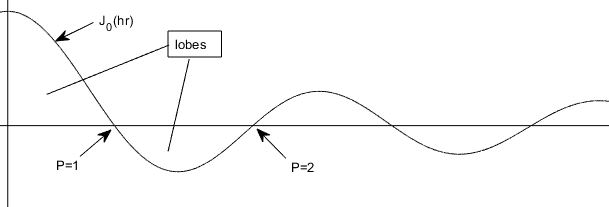
\includegraphics[width=1\linewidth]{\pathtoparttwo/graphics/fig_6.1}
\caption{Plot of the roots of the Bessel function $J_0(hr)$}
\label{fig:fig6}
\end{figure}

Therefore $J_n^p(hr)$ corresponds to TM$_{np}$ mode where n tells us the number of wavelengths $\lambda$ that is in the $\phi$ direction and p tells us the number of lobes that is in the r direction.

The fundamental TM mode in the TM$_{01}$ mode which has 
$$
ha = 2.405 \Longrightarrow h=\frac{2.405}{a}
$$
from $h^2=\gamma^2+w^2\mu\epsilon $ at cut-off, the propagation constant for a lossless medium is zero since $\gamma=j\beta$ and $\beta=0$ as there is no propagation through the conducting wall. 

So
$$
h^2=\omega_c^2\mu\epsilon
$$ 
where $\omega_c$ is the cut-off frequency in radians given as $2\pi f_c$ and $f_c$ is the cut-off frequency in Hertz.

So $f_c =\frac{h}{2\pi\sqrt{\mu\epsilon}}$, for TM$_{01}$ mode $h=\frac{2.405}{a}$ therefore 
$$
f_c=\frac{2.405}{2\pi a\sqrt{\mu\epsilon}} =\frac{0.383}{a\sqrt{\mu\epsilon}}
$$
The second TM mode is the TM$_{11}$ mode where $ha =3.832$ such that $h=\frac{3.832}{a}$ and $f_c=\frac{3.832}{2\pi a\sqrt{\mu\epsilon}}$. Also, the next mode is the TM$_{21}$ mode for which $ha =5.136$ and $h=\frac{5.136}{a} \Longrightarrow f_c=\frac{5.136}{2\pi a\sqrt{\mu\epsilon}}$ and so on. 

Let's examine the fundamental mode TM$_{01}$ briefly. Here n=0 which implies that only the fields $E_r, E_z$ and $H_\phi$ exist and they are not varying in the $\phi$ direction. They are given as
$$
E_r=\frac{-j\beta}{h^2}C_0J_0'(hr)\\
E_z=C_oJ_o(hr)
$$
and
$$
H_\phi=\frac{j\omega\epsilon}{h^2}C_0J_0'(hr)
$$
From our study of the Bessel function of the first order, $J_0(hr)$ is maximum at hr=0 which is the centre of the waveguide so we expect $E_z$ to vary in the r direction such that it is maximum at the centre and it reduces to zero for the first root at the surface. The two-dimensional plots will be treated in the next lecture for different TM modes where we can visually see the changes in the magnitudes of fields in the waveguide.
